% Options for packages loaded elsewhere
% Options for packages loaded elsewhere
\PassOptionsToPackage{unicode}{hyperref}
\PassOptionsToPackage{hyphens}{url}
\PassOptionsToPackage{dvipsnames,svgnames,x11names}{xcolor}
%
\documentclass[
  letterpaper,
  DIV=11,
  numbers=noendperiod]{scrreprt}
\usepackage{xcolor}
\usepackage{amsmath,amssymb}
\setcounter{secnumdepth}{5}
\usepackage{iftex}
\ifPDFTeX
  \usepackage[T1]{fontenc}
  \usepackage[utf8]{inputenc}
  \usepackage{textcomp} % provide euro and other symbols
\else % if luatex or xetex
  \usepackage{unicode-math} % this also loads fontspec
  \defaultfontfeatures{Scale=MatchLowercase}
  \defaultfontfeatures[\rmfamily]{Ligatures=TeX,Scale=1}
\fi
\usepackage{lmodern}
\ifPDFTeX\else
  % xetex/luatex font selection
\fi
% Use upquote if available, for straight quotes in verbatim environments
\IfFileExists{upquote.sty}{\usepackage{upquote}}{}
\IfFileExists{microtype.sty}{% use microtype if available
  \usepackage[]{microtype}
  \UseMicrotypeSet[protrusion]{basicmath} % disable protrusion for tt fonts
}{}
\makeatletter
\@ifundefined{KOMAClassName}{% if non-KOMA class
  \IfFileExists{parskip.sty}{%
    \usepackage{parskip}
  }{% else
    \setlength{\parindent}{0pt}
    \setlength{\parskip}{6pt plus 2pt minus 1pt}}
}{% if KOMA class
  \KOMAoptions{parskip=half}}
\makeatother
% Make \paragraph and \subparagraph free-standing
\makeatletter
\ifx\paragraph\undefined\else
  \let\oldparagraph\paragraph
  \renewcommand{\paragraph}{
    \@ifstar
      \xxxParagraphStar
      \xxxParagraphNoStar
  }
  \newcommand{\xxxParagraphStar}[1]{\oldparagraph*{#1}\mbox{}}
  \newcommand{\xxxParagraphNoStar}[1]{\oldparagraph{#1}\mbox{}}
\fi
\ifx\subparagraph\undefined\else
  \let\oldsubparagraph\subparagraph
  \renewcommand{\subparagraph}{
    \@ifstar
      \xxxSubParagraphStar
      \xxxSubParagraphNoStar
  }
  \newcommand{\xxxSubParagraphStar}[1]{\oldsubparagraph*{#1}\mbox{}}
  \newcommand{\xxxSubParagraphNoStar}[1]{\oldsubparagraph{#1}\mbox{}}
\fi
\makeatother

\usepackage{color}
\usepackage{fancyvrb}
\newcommand{\VerbBar}{|}
\newcommand{\VERB}{\Verb[commandchars=\\\{\}]}
\DefineVerbatimEnvironment{Highlighting}{Verbatim}{commandchars=\\\{\}}
% Add ',fontsize=\small' for more characters per line
\usepackage{framed}
\definecolor{shadecolor}{RGB}{241,243,245}
\newenvironment{Shaded}{\begin{snugshade}}{\end{snugshade}}
\newcommand{\AlertTok}[1]{\textcolor[rgb]{0.68,0.00,0.00}{#1}}
\newcommand{\AnnotationTok}[1]{\textcolor[rgb]{0.37,0.37,0.37}{#1}}
\newcommand{\AttributeTok}[1]{\textcolor[rgb]{0.40,0.45,0.13}{#1}}
\newcommand{\BaseNTok}[1]{\textcolor[rgb]{0.68,0.00,0.00}{#1}}
\newcommand{\BuiltInTok}[1]{\textcolor[rgb]{0.00,0.23,0.31}{#1}}
\newcommand{\CharTok}[1]{\textcolor[rgb]{0.13,0.47,0.30}{#1}}
\newcommand{\CommentTok}[1]{\textcolor[rgb]{0.37,0.37,0.37}{#1}}
\newcommand{\CommentVarTok}[1]{\textcolor[rgb]{0.37,0.37,0.37}{\textit{#1}}}
\newcommand{\ConstantTok}[1]{\textcolor[rgb]{0.56,0.35,0.01}{#1}}
\newcommand{\ControlFlowTok}[1]{\textcolor[rgb]{0.00,0.23,0.31}{\textbf{#1}}}
\newcommand{\DataTypeTok}[1]{\textcolor[rgb]{0.68,0.00,0.00}{#1}}
\newcommand{\DecValTok}[1]{\textcolor[rgb]{0.68,0.00,0.00}{#1}}
\newcommand{\DocumentationTok}[1]{\textcolor[rgb]{0.37,0.37,0.37}{\textit{#1}}}
\newcommand{\ErrorTok}[1]{\textcolor[rgb]{0.68,0.00,0.00}{#1}}
\newcommand{\ExtensionTok}[1]{\textcolor[rgb]{0.00,0.23,0.31}{#1}}
\newcommand{\FloatTok}[1]{\textcolor[rgb]{0.68,0.00,0.00}{#1}}
\newcommand{\FunctionTok}[1]{\textcolor[rgb]{0.28,0.35,0.67}{#1}}
\newcommand{\ImportTok}[1]{\textcolor[rgb]{0.00,0.46,0.62}{#1}}
\newcommand{\InformationTok}[1]{\textcolor[rgb]{0.37,0.37,0.37}{#1}}
\newcommand{\KeywordTok}[1]{\textcolor[rgb]{0.00,0.23,0.31}{\textbf{#1}}}
\newcommand{\NormalTok}[1]{\textcolor[rgb]{0.00,0.23,0.31}{#1}}
\newcommand{\OperatorTok}[1]{\textcolor[rgb]{0.37,0.37,0.37}{#1}}
\newcommand{\OtherTok}[1]{\textcolor[rgb]{0.00,0.23,0.31}{#1}}
\newcommand{\PreprocessorTok}[1]{\textcolor[rgb]{0.68,0.00,0.00}{#1}}
\newcommand{\RegionMarkerTok}[1]{\textcolor[rgb]{0.00,0.23,0.31}{#1}}
\newcommand{\SpecialCharTok}[1]{\textcolor[rgb]{0.37,0.37,0.37}{#1}}
\newcommand{\SpecialStringTok}[1]{\textcolor[rgb]{0.13,0.47,0.30}{#1}}
\newcommand{\StringTok}[1]{\textcolor[rgb]{0.13,0.47,0.30}{#1}}
\newcommand{\VariableTok}[1]{\textcolor[rgb]{0.07,0.07,0.07}{#1}}
\newcommand{\VerbatimStringTok}[1]{\textcolor[rgb]{0.13,0.47,0.30}{#1}}
\newcommand{\WarningTok}[1]{\textcolor[rgb]{0.37,0.37,0.37}{\textit{#1}}}

\usepackage{longtable,booktabs,array}
\usepackage{calc} % for calculating minipage widths
% Correct order of tables after \paragraph or \subparagraph
\usepackage{etoolbox}
\makeatletter
\patchcmd\longtable{\par}{\if@noskipsec\mbox{}\fi\par}{}{}
\makeatother
% Allow footnotes in longtable head/foot
\IfFileExists{footnotehyper.sty}{\usepackage{footnotehyper}}{\usepackage{footnote}}
\makesavenoteenv{longtable}
\usepackage{graphicx}
\makeatletter
\newsavebox\pandoc@box
\newcommand*\pandocbounded[1]{% scales image to fit in text height/width
  \sbox\pandoc@box{#1}%
  \Gscale@div\@tempa{\textheight}{\dimexpr\ht\pandoc@box+\dp\pandoc@box\relax}%
  \Gscale@div\@tempb{\linewidth}{\wd\pandoc@box}%
  \ifdim\@tempb\p@<\@tempa\p@\let\@tempa\@tempb\fi% select the smaller of both
  \ifdim\@tempa\p@<\p@\scalebox{\@tempa}{\usebox\pandoc@box}%
  \else\usebox{\pandoc@box}%
  \fi%
}
% Set default figure placement to htbp
\def\fps@figure{htbp}
\makeatother





\setlength{\emergencystretch}{3em} % prevent overfull lines

\providecommand{\tightlist}{%
  \setlength{\itemsep}{0pt}\setlength{\parskip}{0pt}}



 


\KOMAoption{captions}{tableheading}
\makeatletter
\@ifpackageloaded{tcolorbox}{}{\usepackage[skins,breakable]{tcolorbox}}
\@ifpackageloaded{fontawesome5}{}{\usepackage{fontawesome5}}
\definecolor{quarto-callout-color}{HTML}{909090}
\definecolor{quarto-callout-note-color}{HTML}{0758E5}
\definecolor{quarto-callout-important-color}{HTML}{CC1914}
\definecolor{quarto-callout-warning-color}{HTML}{EB9113}
\definecolor{quarto-callout-tip-color}{HTML}{00A047}
\definecolor{quarto-callout-caution-color}{HTML}{FC5300}
\definecolor{quarto-callout-color-frame}{HTML}{acacac}
\definecolor{quarto-callout-note-color-frame}{HTML}{4582ec}
\definecolor{quarto-callout-important-color-frame}{HTML}{d9534f}
\definecolor{quarto-callout-warning-color-frame}{HTML}{f0ad4e}
\definecolor{quarto-callout-tip-color-frame}{HTML}{02b875}
\definecolor{quarto-callout-caution-color-frame}{HTML}{fd7e14}
\makeatother
\makeatletter
\@ifpackageloaded{bookmark}{}{\usepackage{bookmark}}
\makeatother
\makeatletter
\@ifpackageloaded{caption}{}{\usepackage{caption}}
\AtBeginDocument{%
\ifdefined\contentsname
  \renewcommand*\contentsname{Table of contents}
\else
  \newcommand\contentsname{Table of contents}
\fi
\ifdefined\listfigurename
  \renewcommand*\listfigurename{List of Figures}
\else
  \newcommand\listfigurename{List of Figures}
\fi
\ifdefined\listtablename
  \renewcommand*\listtablename{List of Tables}
\else
  \newcommand\listtablename{List of Tables}
\fi
\ifdefined\figurename
  \renewcommand*\figurename{Figure}
\else
  \newcommand\figurename{Figure}
\fi
\ifdefined\tablename
  \renewcommand*\tablename{Table}
\else
  \newcommand\tablename{Table}
\fi
}
\@ifpackageloaded{float}{}{\usepackage{float}}
\floatstyle{ruled}
\@ifundefined{c@chapter}{\newfloat{codelisting}{h}{lop}}{\newfloat{codelisting}{h}{lop}[chapter]}
\floatname{codelisting}{Listing}
\newcommand*\listoflistings{\listof{codelisting}{List of Listings}}
\makeatother
\makeatletter
\makeatother
\makeatletter
\@ifpackageloaded{caption}{}{\usepackage{caption}}
\@ifpackageloaded{subcaption}{}{\usepackage{subcaption}}
\makeatother
\usepackage{bookmark}
\IfFileExists{xurl.sty}{\usepackage{xurl}}{} % add URL line breaks if available
\urlstyle{same}
\hypersetup{
  pdftitle={STAT 8670 - Computational Methods in Statistics},
  pdfauthor={Chi-Kuang Yeh},
  colorlinks=true,
  linkcolor={blue},
  filecolor={Maroon},
  citecolor={Blue},
  urlcolor={Blue},
  pdfcreator={LaTeX via pandoc}}


\title{STAT 8670 - Computational Methods in Statistics}
\author{Chi-Kuang Yeh}
\date{2025-09-03}
\begin{document}
\maketitle

\renewcommand*\contentsname{Table of contents}
{
\hypersetup{linkcolor=}
\setcounter{tocdepth}{2}
\tableofcontents
}

\bookmarksetup{startatroot}

\chapter*{Preface}\label{preface}
\addcontentsline{toc}{chapter}{Preface}

\markboth{Preface}{Preface}

\section*{Description}\label{description}
\addcontentsline{toc}{section}{Description}

\markright{Description}

Topics ins included are optimization, numerical integration,
bootstrapping, cross-validation and Jackknife, density estimation,
smoothing, and use of the statistical computer package of S-plus/R.

\subsection*{Prerequisites}\label{prerequisites}
\addcontentsline{toc}{subsection}{Prerequisites}

MATH 4752/6752 -- Mathematical Statistics II, and the ability to program
in a high-level language.

\subsection*{Instructor}\label{instructor}
\addcontentsline{toc}{subsection}{Instructor}

\href{https://chikuang.github.io/}{Chi-Kuang Yeh}, I am an Assistant
Professor in the Department of Mathematics and Statistics, Georgia State
University.

\begin{itemize}
\tightlist
\item
  Office: Suite 1407, 25 Park Place.
\item
  Email: \href{mailto:cyeh@gsu.edu}{\nolinkurl{cyeh@gsu.edu}}.
\end{itemize}

\section*{Office Hour}\label{office-hour}
\addcontentsline{toc}{section}{Office Hour}

\markright{Office Hour}

14:00--15:00 on Tuesday and Wednesday.

\section*{Assignment}\label{assignment}
\addcontentsline{toc}{section}{Assignment}

\markright{Assignment}

\begin{itemize}
\tightlist
\item[$\square$]
  Assignment 1: Date and topics TBA
\end{itemize}

\section*{Midterm}\label{midterm}
\addcontentsline{toc}{section}{Midterm}

\markright{Midterm}

\begin{itemize}
\tightlist
\item[$\square$]
  Midterm 1: Date and topics TBA
\item[$\square$]
  Midterm 2: Date and topics TBA
\end{itemize}

\section*{Final Exam}\label{final-exam}
\addcontentsline{toc}{section}{Final Exam}

\markright{Final Exam}

\begin{itemize}
\tightlist
\item[$\square$]
  Final Project: Date and topics TBA
\end{itemize}

\section*{Topics and Corresponding
Lectures}\label{topics-and-corresponding-lectures}
\addcontentsline{toc}{section}{Topics and Corresponding Lectures}

\markright{Topics and Corresponding Lectures}

Those chapters are based on the lecture notes. This part will be updated
frequently.

\begin{longtable}[]{@{}lc@{}}
\toprule\noalign{}
Topic & Lecture Covered \\
\midrule\noalign{}
\endhead
\bottomrule\noalign{}
\endlastfoot
Introduction to R Programming & 1--2 \\
Optimization & 3-- \\
Numerical integration & TBA \\
Jackknife & TBA \\
Bootstrap & TBA \\
Cross-validation & TBA \\
Smoothing & TBA \\
Density estimation & TBA \\
Monte Carlo Methods & TBA \\
\end{longtable}

\section*{Recommended Textbooks}\label{recommended-textbooks}
\addcontentsline{toc}{section}{Recommended Textbooks}

\markright{Recommended Textbooks}

\begin{itemize}
\item
  Givens, G.H. and Hoeting, J.A. (2012).
  \href{https://www.stat.colostate.edu/computationalstatistics/}{\emph{Computational
  Statistics}}. Wiley, New York.
\item
  Rizzo, M.L. (2007)
  \href{https://a-roshani.ir/files/SC/\%5B4\%5D\%20\%5BMaria\%20L.\%20Rizzo\%5D\%5B2019\%5D\%20Statistical\%20Computing\%20\%20with\%20R,\%20Second\%20Edition.pdf}{\emph{Statistical
  Computing with R}}. CRC Press, Roca Baton.
\item
  Hothorn, T. and Everitt, B.S. (2006).
  \href{https://digitallibrary.tsu.ge/book/2019/september/books/A-Handbook-of-Statistical-Analyses.pdf}{\emph{A
  Handbook of Statistical Analyses Using R}}. CRC Press, Boca Raton.
\end{itemize}

\section*{Side Readings}\label{side-readings}
\addcontentsline{toc}{section}{Side Readings}

\markright{Side Readings}

\begin{itemize}
\tightlist
\item
  Wickham, H., Çetinkaya-Rundel, M. and Grolemund, G. (2023).
  \href{https://r4ds.hadley.nz/}{\emph{R for Data Science}}. O'Reilly.
\end{itemize}

\bookmarksetup{startatroot}

\chapter{Data Structure and R
Programming}\label{data-structure-and-r-programming}

Data types, operators, variables

Two basic types of objects: (1) data \& (2) functions

\begin{itemize}
\item
  Data: can be a number, a vector, a matrix, a dataframe, a list or
  other datatypes
\item
  Function: a function is a set of instructions that takes input,
  processes it, and returns output. Functions can be built-in or
  user-defined.
\end{itemize}

\section{Data type}\label{data-type}

\begin{itemize}
\item
  Boolean/Logical: Yes or No, Head or Tail, True or False
\item
  Integers: Whole numbers \(\mathbb{Z}\), e.g., 1, 2, 3, -1, -2, -3
\item
  Characters: Text strings, e.g., ``Hello'', ``World.''
\item
  Floats: Noninteger fractional numbers, e.g., \(\pi\), \(e\).
\item
  Missing data: \texttt{NA} in R, which stands for ``Not Available.'' It
  is used to represent missing or undefined values in a dataset.
\end{itemize}

\begin{Shaded}
\begin{Highlighting}[]
\NormalTok{day }\OtherTok{\textless{}{-}} \FunctionTok{c}\NormalTok{(}\StringTok{"Monday"}\NormalTok{, }\StringTok{"Tuesday"}\NormalTok{, }\StringTok{"Wednesday"}\NormalTok{, }\StringTok{"Thursday"}\NormalTok{, }\StringTok{"Friday"}\NormalTok{)}
\NormalTok{weather }\OtherTok{\textless{}{-}} \FunctionTok{c}\NormalTok{(}\StringTok{"Raining"}\NormalTok{, }\StringTok{"Sunny"}\NormalTok{, }\ConstantTok{NA}\NormalTok{, }\StringTok{"Windy"}\NormalTok{, }\StringTok{"Snowing"}\NormalTok{)}
\FunctionTok{data.frame}\NormalTok{(}\FunctionTok{rbind}\NormalTok{(day, weather))}
\end{Highlighting}
\end{Shaded}

\begin{verbatim}
             X1      X2        X3       X4      X5
day      Monday Tuesday Wednesday Thursday  Friday
weather Raining   Sunny      <NA>    Windy Snowing
\end{verbatim}

\begin{itemize}
\tightlist
\item
  Other more complex types
\end{itemize}

\subsection{To change data type}\label{to-change-data-type}

You may change the data type using the following functions, but the
chance is that some of the information will be missing. Do this with
caution!

\begin{Shaded}
\begin{Highlighting}[]
\NormalTok{x }\OtherTok{\textless{}{-}}\NormalTok{ pi}
\FunctionTok{print}\NormalTok{(x)}
\end{Highlighting}
\end{Shaded}

\begin{verbatim}
[1] 3.141593
\end{verbatim}

\begin{Shaded}
\begin{Highlighting}[]
\NormalTok{x\_int }\OtherTok{\textless{}{-}} \FunctionTok{as.integer}\NormalTok{(x)}
\FunctionTok{print}\NormalTok{(x\_int)}
\end{Highlighting}
\end{Shaded}

\begin{verbatim}
[1] 3
\end{verbatim}

Some of the conversion functions:

\begin{itemize}
\tightlist
\item
  \texttt{as.integer()}: Convert to integer.
\item
  \texttt{as.numeric()}: Convert to numeric (float).
\item
  \texttt{as.character()}: Convert to character.
\item
  \texttt{as.logical()}: Convert to logical (boolean).
\item
  \texttt{as.Date()}: Convert to date.
\item
  \texttt{as.factor()}: Convert to factor (categorical variable).
\item
  \texttt{as.list()}: Convert to list.
\item
  \texttt{as.matrix()}: Convert to matrix.
\item
  \texttt{as.data.frame()}: Convert to data frame.
\item
  \texttt{as.vector()}: Convert to vector.
\item
  \texttt{as.complex()}: Convert to complex number.
\end{itemize}

\section{Operators}\label{operators}

\begin{itemize}
\item
  Unary: With only \textbf{one} argument. E.g., \texttt{-x} (negation),
  \texttt{!x} (logical negation).
\item
  Binary: With \textbf{two} arguments. E.g., \texttt{x\ +\ y}
  (addition), \texttt{x\ -\ y} (subtraction), \texttt{x\ *\ y}
  (multiplication), \texttt{x\ /\ y} (division).
\end{itemize}

\subsection{Comparison Operator}\label{comparison-operator}

Comparing two objects. E.g., \texttt{x\ ==\ y} (equal),
\texttt{x\ !=\ y} (not equal), \texttt{x\ \textless{}\ y} (less than),
\texttt{x\ \textgreater{}\ y} (greater than),
\texttt{x\ \textless{}=\ y} (less than or equal to),
\texttt{x\ \textgreater{}=\ y} (greater than or equal to).

\subsection{Logical Operator}\label{logical-operator}

Logical operators are used to combine or manipulate logical values (TRUE
or FALSE). E.g., \texttt{x\ \&\ y} (logical AND),
\texttt{x\ \textbar{}\ y} (logical OR), \texttt{!x} (logical NOT).

We shall note that the logical operators in R are vectorized,
\texttt{x\ \textbar{}\ y} and \texttt{x\ \textbar{}\textbar{}\ y} are
different. The former is vectorized, while the latter is not.

\begin{Shaded}
\begin{Highlighting}[]
\NormalTok{x }\OtherTok{\textless{}{-}} \FunctionTok{c}\NormalTok{(}\ConstantTok{TRUE}\NormalTok{, }\ConstantTok{FALSE}\NormalTok{, }\ConstantTok{FALSE}\NormalTok{)}
\NormalTok{y }\OtherTok{\textless{}{-}} \FunctionTok{c}\NormalTok{(}\ConstantTok{TRUE}\NormalTok{, }\ConstantTok{FALSE}\NormalTok{, }\ConstantTok{FALSE}\NormalTok{)}
\NormalTok{x }\SpecialCharTok{|}\NormalTok{ y  }\CommentTok{\# [1]  TRUE FALSE FALSE}
\NormalTok{x }\SpecialCharTok{||}\NormalTok{ y }\CommentTok{\# This will return an error}
\end{Highlighting}
\end{Shaded}

\section{Indexing}\label{indexing}

Indexing is a way to access or modify specific elements in a data
structure. In \textbf{R}, indexing can be done using square brackets
\texttt{{[}{]}} for vectors and matrices, or the \texttt{\$} operator
for data frames. Note that the index starts from \textbf{0} in
\textbf{R}, which is different from some other programming languages
like Python.

\section{Naming}\label{naming}

In \textbf{R}, you can assign names to objects using the
\texttt{names()} function. This is useful for making your code more
readable and for accessing specific elements in a data structure.

A good practice is to use \texttt{\_} (underscore) to separate words in
variable names, e.g., \texttt{my\_variable}. This makes the code more
readable and easier to understand.

\begin{Shaded}
\begin{Highlighting}[]
\CommentTok{\# Assign names to a vector}
\NormalTok{temp }\OtherTok{\textless{}{-}} \FunctionTok{c}\NormalTok{(}\DecValTok{20}\NormalTok{, }\DecValTok{30}\NormalTok{, }\DecValTok{27}\NormalTok{, }\DecValTok{31}\NormalTok{, }\DecValTok{45}\NormalTok{)}
\FunctionTok{names}\NormalTok{(temp) }\OtherTok{\textless{}{-}} \FunctionTok{c}\NormalTok{(}\StringTok{"Mon"}\NormalTok{, }\StringTok{"Tues"}\NormalTok{, }\StringTok{"Wed"}\NormalTok{, }\StringTok{"Thurs"}\NormalTok{, }\StringTok{"Fri"}\NormalTok{)}
\FunctionTok{print}\NormalTok{(temp)}
\end{Highlighting}
\end{Shaded}

\begin{verbatim}
  Mon  Tues   Wed Thurs   Fri 
   20    30    27    31    45 
\end{verbatim}

\begin{Shaded}
\begin{Highlighting}[]
\FunctionTok{rownames}\NormalTok{(temp) }\OtherTok{\textless{}{-}} \StringTok{"Day1"} \CommentTok{\# error}
\end{Highlighting}
\end{Shaded}

\begin{Shaded}
\begin{Highlighting}[]
\NormalTok{temp\_mat }\OtherTok{\textless{}{-}} \FunctionTok{matrix}\NormalTok{(}\FunctionTok{c}\NormalTok{(}\DecValTok{20}\NormalTok{, }\DecValTok{30}\NormalTok{, }\DecValTok{27}\NormalTok{, }\DecValTok{31}\NormalTok{, }\DecValTok{45}\NormalTok{), }\AttributeTok{nrow =} \DecValTok{1}\NormalTok{, }\AttributeTok{ncol =} \DecValTok{5}\NormalTok{)}
\FunctionTok{colnames}\NormalTok{(temp\_mat) }\OtherTok{\textless{}{-}} \FunctionTok{c}\NormalTok{(}\StringTok{"Mon"}\NormalTok{, }\StringTok{"Tues"}\NormalTok{, }\StringTok{"Wed"}\NormalTok{, }\StringTok{"Thurs"}\NormalTok{, }\StringTok{"Fri"}\NormalTok{)}
\FunctionTok{rownames}\NormalTok{(temp\_mat) }\OtherTok{\textless{}{-}} \StringTok{"Day1"} \CommentTok{\# error}
\FunctionTok{print}\NormalTok{(temp\_mat)}
\end{Highlighting}
\end{Shaded}

\begin{verbatim}
     Mon Tues Wed Thurs Fri
Day1  20   30  27    31  45
\end{verbatim}

\section{Array and Matrix}\label{array-and-matrix}

One may define an array or a matrix in \textbf{R} using the
\texttt{array()} or \texttt{matrix()} functions, respectively. An array
is a multi-dimensional data structure, while a matrix is a
two-dimensional array.

\begin{Shaded}
\begin{Highlighting}[]
\CommentTok{\# Create a 1{-}dimensional array}
\NormalTok{array\_1d }\OtherTok{\textless{}{-}} \FunctionTok{array}\NormalTok{(}\DecValTok{1}\SpecialCharTok{:}\DecValTok{10}\NormalTok{, }\AttributeTok{dim =} \DecValTok{10}\NormalTok{)}
\NormalTok{array\_1d}
\end{Highlighting}
\end{Shaded}

\begin{verbatim}
 [1]  1  2  3  4  5  6  7  8  9 10
\end{verbatim}

\begin{Shaded}
\begin{Highlighting}[]
\CommentTok{\# Create a 2{-}dimensional array}
\NormalTok{array\_2d }\OtherTok{\textless{}{-}} \FunctionTok{array}\NormalTok{(}\DecValTok{1}\SpecialCharTok{:}\DecValTok{12}\NormalTok{, }\AttributeTok{dim =} \FunctionTok{c}\NormalTok{(}\DecValTok{4}\NormalTok{, }\DecValTok{3}\NormalTok{))}
\NormalTok{array\_2d}
\end{Highlighting}
\end{Shaded}

\begin{verbatim}
     [,1] [,2] [,3]
[1,]    1    5    9
[2,]    2    6   10
[3,]    3    7   11
[4,]    4    8   12
\end{verbatim}

\begin{Shaded}
\begin{Highlighting}[]
\CommentTok{\# Create a 3{-}dimensional array}
\NormalTok{array\_3d }\OtherTok{\textless{}{-}} \FunctionTok{array}\NormalTok{(}\DecValTok{1}\SpecialCharTok{:}\DecValTok{24}\NormalTok{, }\AttributeTok{dim =} \FunctionTok{c}\NormalTok{(}\DecValTok{4}\NormalTok{, }\DecValTok{3}\NormalTok{, }\DecValTok{2}\NormalTok{))}
\NormalTok{array\_3d}
\end{Highlighting}
\end{Shaded}

\begin{verbatim}
, , 1

     [,1] [,2] [,3]
[1,]    1    5    9
[2,]    2    6   10
[3,]    3    7   11
[4,]    4    8   12

, , 2

     [,1] [,2] [,3]
[1,]   13   17   21
[2,]   14   18   22
[3,]   15   19   23
[4,]   16   20   24
\end{verbatim}

\begin{Shaded}
\begin{Highlighting}[]
\CommentTok{\# Create a matrix}
\NormalTok{my\_matrix }\OtherTok{\textless{}{-}} \FunctionTok{matrix}\NormalTok{(}\DecValTok{1}\SpecialCharTok{:}\DecValTok{12}\NormalTok{, }\AttributeTok{nrow =} \DecValTok{4}\NormalTok{, }\AttributeTok{ncol =} \DecValTok{3}\NormalTok{)}
\NormalTok{my\_matrix}
\end{Highlighting}
\end{Shaded}

\begin{verbatim}
     [,1] [,2] [,3]
[1,]    1    5    9
[2,]    2    6   10
[3,]    3    7   11
[4,]    4    8   12
\end{verbatim}

Note here, the matrix is a special case of an array, where the number of
dimensions is exactly 2.

\begin{Shaded}
\begin{Highlighting}[]
\FunctionTok{is.matrix}\NormalTok{(array\_2d)   }\CommentTok{\# TRUE}
\FunctionTok{is.matrix}\NormalTok{(my\_matrix)  }\CommentTok{\# TRUE}

\FunctionTok{is.array}\NormalTok{(array\_2d)    }\CommentTok{\# TRUE}
\FunctionTok{is.array}\NormalTok{(my\_matrix)   }\CommentTok{\# TRUE}
\end{Highlighting}
\end{Shaded}

\section{Key and Value Pair}\label{key-and-value-pair}

Key-Value Pair is a data structure that consists of a key and its
corresponding value. In \textbf{R}, this can be implemented using named
vectors, lists, or data frames. Usually, the most commonly used case is
in the lists and data frames. The values can be extra by providing the
corresonding key

\begin{Shaded}
\begin{Highlighting}[]
\NormalTok{key1 }\OtherTok{\textless{}{-}} \StringTok{"Tues"}
\NormalTok{value1 }\OtherTok{\textless{}{-}} \DecValTok{32}
\NormalTok{key2 }\OtherTok{\textless{}{-}} \StringTok{"Wed"}
\NormalTok{value2 }\OtherTok{\textless{}{-}} \DecValTok{28}

\NormalTok{list\_temp }\OtherTok{\textless{}{-}} \FunctionTok{list}\NormalTok{()}
\NormalTok{list\_temp[[ key1 ]] }\OtherTok{\textless{}{-}}\NormalTok{ value1}
\NormalTok{list\_temp[[ key2 ]] }\OtherTok{\textless{}{-}}\NormalTok{ value2}

\FunctionTok{print}\NormalTok{(list\_temp)}
\end{Highlighting}
\end{Shaded}

\begin{verbatim}
$Tues
[1] 32

$Wed
[1] 28
\end{verbatim}

\begin{Shaded}
\begin{Highlighting}[]
\DocumentationTok{\#\# Now providing a key {-} Tues}
\DocumentationTok{\#\#\# First way}
\NormalTok{list\_temp[[}\StringTok{"Tues"}\NormalTok{]]}
\end{Highlighting}
\end{Shaded}

\begin{verbatim}
[1] 32
\end{verbatim}

\begin{Shaded}
\begin{Highlighting}[]
\DocumentationTok{\#\#\# Second way}
\NormalTok{list\_temp}\SpecialCharTok{$}\NormalTok{Tues}
\end{Highlighting}
\end{Shaded}

\begin{verbatim}
[1] 32
\end{verbatim}

\section{Data Frame}\label{data-frame}

Dataframe is a two-dimensional, tabular data structure in R that can
hold different types of variables (numeric, character, factor, etc.) in
each column. It is similar to a spreadsheet or SQL table.

\begin{Shaded}
\begin{Highlighting}[]
\NormalTok{iris }\OtherTok{\textless{}{-}}\NormalTok{ datasets}\SpecialCharTok{::}\NormalTok{iris}
\FunctionTok{head}\NormalTok{(iris)}
\end{Highlighting}
\end{Shaded}

\begin{verbatim}
  Sepal.Length Sepal.Width Petal.Length Petal.Width Species
1          5.1         3.5          1.4         0.2  setosa
2          4.9         3.0          1.4         0.2  setosa
3          4.7         3.2          1.3         0.2  setosa
4          4.6         3.1          1.5         0.2  setosa
5          5.0         3.6          1.4         0.2  setosa
6          5.4         3.9          1.7         0.4  setosa
\end{verbatim}

\section{Apply function}\label{apply-function}

The \texttt{apply()} function is the basic model of the family of apply
functions in R, which includes specific functions like
\texttt{lapply()}, \texttt{sapply()}, \texttt{tapply()},
\texttt{mapply()}, \texttt{vapply()}, \texttt{rapply()},
\texttt{bapply()}, \texttt{eapply()}, and others. These functions are
used to apply a function to elements of a data structure (like a vector,
list, or data frame) in a (sometimes) more efficient and concise way
than using loops.

\begin{Shaded}
\begin{Highlighting}[]
\NormalTok{x }\OtherTok{\textless{}{-}} \FunctionTok{cbind}\NormalTok{(}\AttributeTok{x1 =} \DecValTok{3}\NormalTok{, }\AttributeTok{x2 =} \FunctionTok{c}\NormalTok{(}\DecValTok{4}\SpecialCharTok{:}\DecValTok{1}\NormalTok{, }\DecValTok{2}\SpecialCharTok{:}\DecValTok{5}\NormalTok{))}
\FunctionTok{dimnames}\NormalTok{(x)[[}\DecValTok{1}\NormalTok{]] }\OtherTok{\textless{}{-}}\NormalTok{ letters[}\DecValTok{1}\SpecialCharTok{:}\DecValTok{8}\NormalTok{]}
\FunctionTok{print}\NormalTok{(x)}
\end{Highlighting}
\end{Shaded}

\begin{verbatim}
  x1 x2
a  3  4
b  3  3
c  3  2
d  3  1
e  3  2
f  3  3
g  3  4
h  3  5
\end{verbatim}

\begin{Shaded}
\begin{Highlighting}[]
\FunctionTok{apply}\NormalTok{(x, }\AttributeTok{MARGIN =} \DecValTok{2}\NormalTok{, mean) }\CommentTok{\#apply the mean function to their "columns"}
\end{Highlighting}
\end{Shaded}

\begin{verbatim}
x1 x2 
 3  3 
\end{verbatim}

\begin{Shaded}
\begin{Highlighting}[]
\NormalTok{col.sums }\OtherTok{\textless{}{-}} \FunctionTok{apply}\NormalTok{(x, }\AttributeTok{MARGIN =} \DecValTok{2}\NormalTok{, sum) }\CommentTok{\#apply the sum function to their "columns"}
\NormalTok{row.sums }\OtherTok{\textless{}{-}} \FunctionTok{apply}\NormalTok{(x, }\AttributeTok{MARGIN =} \DecValTok{1}\NormalTok{, sum) }\CommentTok{\#apply the sum function to their "rows"}
\FunctionTok{rbind}\NormalTok{(}\FunctionTok{cbind}\NormalTok{(x, }\AttributeTok{Rtot =}\NormalTok{ row.sums), }\AttributeTok{Ctot =} \FunctionTok{c}\NormalTok{(col.sums, }\FunctionTok{sum}\NormalTok{(col.sums)))}
\end{Highlighting}
\end{Shaded}

\begin{verbatim}
     x1 x2 Rtot
a     3  4    7
b     3  3    6
c     3  2    5
d     3  1    4
e     3  2    5
f     3  3    6
g     3  4    7
h     3  5    8
Ctot 24 24   48
\end{verbatim}

Some of the commonly used apply functions:

\begin{itemize}
\item
  \textbf{lapply}: Apply a Function over a List or Vector
\item
  \textbf{sapply}: a user-friendly version and wrapper of lapply by
  default returning a vector, matrix
\item
  \textbf{vapply}: similar to sapply, but has a pre-specified type of
  return value, so it can be safer (and sometimes faster) to use.
\end{itemize}

\section{Tidyverse}\label{tidyverse}

The tidyverse is a collection of open source packages for the R
programming language introduced by Hadley Wickham and his team that
``share an underlying design philosophy, grammar, and data structures''
of tidy data. Characteristic features of tidyverse packages include
extensive use of non-standard evaluation and encouraging piping.

\begin{Shaded}
\begin{Highlighting}[]
\DocumentationTok{\#\# Load all tidyverse packages}
\FunctionTok{library}\NormalTok{(tidyverse)}
\end{Highlighting}
\end{Shaded}

\begin{verbatim}
-- Attaching core tidyverse packages ------------------------ tidyverse 2.0.0 --
v dplyr     1.1.4     v readr     2.1.5
v forcats   1.0.0     v stringr   1.5.1
v ggplot2   3.5.2     v tibble    3.3.0
v lubridate 1.9.4     v tidyr     1.3.1
v purrr     1.1.0     
-- Conflicts ------------------------------------------ tidyverse_conflicts() --
x dplyr::filter() masks stats::filter()
x dplyr::lag()    masks stats::lag()
i Use the conflicted package (<http://conflicted.r-lib.org/>) to force all conflicts to become errors
\end{verbatim}

\begin{Shaded}
\begin{Highlighting}[]
\DocumentationTok{\#\# Or load specific packages in the tidy family}
\FunctionTok{library}\NormalTok{(dplyr) }\CommentTok{\# Data manipulation}
\FunctionTok{library}\NormalTok{(ggplot2) }\CommentTok{\# Data visualization}
\FunctionTok{library}\NormalTok{(readr) }\CommentTok{\# Data import}
\FunctionTok{library}\NormalTok{(tibble) }\CommentTok{\# Tidy data frames}
\FunctionTok{library}\NormalTok{(tidyr) }\CommentTok{\# Data tidying}
\CommentTok{\# ...}
\end{Highlighting}
\end{Shaded}

\section{Pipe}\label{pipe}

Pipe operator \texttt{\textbar{}\textgreater{}} (native after R version
4.0) or \texttt{\%\textgreater{}\$} (from magrittr package) is a
powerful tool in \textbf{R} that allows you to chain together multiple
operations in a clear and concise way. It takes the output of one
function and passes it as the first argument to the next function.

For example, we can write

\begin{Shaded}
\begin{Highlighting}[]
\FunctionTok{set.seed}\NormalTok{(}\DecValTok{777}\NormalTok{)}
\NormalTok{x }\OtherTok{\textless{}{-}} \FunctionTok{rnorm}\NormalTok{(}\DecValTok{5}\NormalTok{)}

\DocumentationTok{\#\# Without using pipe}
\FunctionTok{print}\NormalTok{(}\FunctionTok{round}\NormalTok{(}\FunctionTok{mean}\NormalTok{(x), }\DecValTok{2}\NormalTok{))}
\end{Highlighting}
\end{Shaded}

\begin{verbatim}
[1] 0.37
\end{verbatim}

\begin{Shaded}
\begin{Highlighting}[]
\DocumentationTok{\#\# Using pipe}
\NormalTok{x }\SpecialCharTok{|\textgreater{}} 
  \FunctionTok{mean}\NormalTok{() }\SpecialCharTok{|\textgreater{}} \CommentTok{\# applying the mean function}
  \FunctionTok{round}\NormalTok{(}\DecValTok{2}\NormalTok{) }\SpecialCharTok{|\textgreater{}} \CommentTok{\#round to 2nd decimal place}
  \FunctionTok{print}\NormalTok{()}
\end{Highlighting}
\end{Shaded}

\begin{verbatim}
[1] 0.37
\end{verbatim}

We can see that, without using the pipe, if we are applying multiple
functions to the same object, we may have hard time to track. This can
make the code less readable and harder to maintain. On the other hand,
using pipe, we can clearly see the sequence of operations being applied
to the data, making it easier to understand and modify.

\subsection{Some rules}\label{some-rules}

\texttt{\textbar{}\textgreater{}} should \textbf{always have a space
before it} and should typically \textbf{be the last thing on a line}.
This simplifies adding new steps, reorganizing existing ones, and
modifying elements within each step.

Note that all of the packages in the tidyverse family support the pipe
operator (except \texttt{ggplot2}!), so you can use it with any of them.

\section{Questions in class}\label{questions-in-class}

\subsection{Lecture 1, August 25, 2025}\label{lecture-1-august-25-2025}

Q1. If I know Python already, why learn R?

Reply: My general take are 1). R is more specialized for statistical
analysis and data visualization, while Python is a more general-purpose
programming language. 2). R has a rich ecosystem of packages and
libraries specifically designed for statistical computing, making it a
popular choice among statisticians and data scientists. 3). R's syntax
and data structures are often more intuitive for statistical tasks,
which can lead to faster development and easier collaboration with other
statisticians. 4). Also, the tidyverse ecosystem including \emph{ggplot}
and others are a big plus when dealing with big dataframes. 5). They are
not meant to replace each other, but work as a complement.

Q2. Why my installation of R sometimes failed on a Windows machine?

Reply: There are many reasons. One of the most common reasons is that
you may need to manually add the path to the environment variable.

\subsection{Lecture 2, August 27, 2025}\label{lecture-2-august-27-2025}

Q1. What's the difference of using \texttt{apply} v.s. \texttt{looping}
in R?

Reply: The apply functions are often faster and more efficient than
looping, especially for large datasets, because they have done some
vectorization under the hood. Also, it has much higher readibility and
better conciseness. However, depends on the task, you may want to do the
\textbf{benchmarking} to see the performance difference.

Q2. How to use \texttt{pipe} with two or more variables?

Reply: There are several ways to do this.

\begin{enumerate}
\def\labelenumi{\arabic{enumi}.}
\tightlist
\item
  Within the tidyverse family: One way is to use the \texttt{dplyr}
  package, which provides a set of functions that work well with the
  pipe operator. For example, you can use the \texttt{mutate()} function
  to create a new variable based on two existing variables. For example,
  you can do
\end{enumerate}

\begin{Shaded}
\begin{Highlighting}[]
\FunctionTok{library}\NormalTok{(dplyr)}
\FunctionTok{library}\NormalTok{(magrittr)  }\CommentTok{\# for \%$\%}
\FunctionTok{library}\NormalTok{(purrr)     }\CommentTok{\# for pmap / exec if needed}

\NormalTok{my\_df }\OtherTok{\textless{}{-}} \FunctionTok{tibble}\NormalTok{(}\AttributeTok{x =} \DecValTok{1}\SpecialCharTok{:}\DecValTok{5}\NormalTok{, }\AttributeTok{y =} \DecValTok{6}\SpecialCharTok{:}\DecValTok{10}\NormalTok{)}
\NormalTok{f  }\OtherTok{\textless{}{-}} \ControlFlowTok{function}\NormalTok{(a, b) a }\SpecialCharTok{+} \DecValTok{2}\SpecialCharTok{*}\NormalTok{b}

\NormalTok{my\_df }\SpecialCharTok{\%\textgreater{}\%}
  \FunctionTok{mutate}\NormalTok{(}\AttributeTok{z =} \FunctionTok{f}\NormalTok{(x, y))}
\end{Highlighting}
\end{Shaded}

\begin{verbatim}
# A tibble: 5 x 3
      x     y     z
  <int> <int> <dbl>
1     1     6    13
2     2     7    16
3     3     8    19
4     4     9    22
5     5    10    25
\end{verbatim}

\begin{enumerate}
\def\labelenumi{\arabic{enumi}.}
\setcounter{enumi}{1}
\tightlist
\item
  Using base R, you may do something like the following through the
  \texttt{magrittr} package's exposition pipe \texttt{\%\$\%}:
\end{enumerate}

\begin{Shaded}
\begin{Highlighting}[]
\FunctionTok{library}\NormalTok{(magrittr)}
\CommentTok{\# method 1}
\NormalTok{my\_df }\SpecialCharTok{\%$\%} \FunctionTok{f}\NormalTok{(x, y) }
\end{Highlighting}
\end{Shaded}

\begin{verbatim}
[1] 13 16 19 22 25
\end{verbatim}

\begin{Shaded}
\begin{Highlighting}[]
\CommentTok{\# or use . as a placeholder}
\CommentTok{\# method 2}
\NormalTok{my\_df }\SpecialCharTok{\%\textgreater{}\%}\NormalTok{ \{ }\FunctionTok{f}\NormalTok{(.}\SpecialCharTok{$}\NormalTok{x, .}\SpecialCharTok{$}\NormalTok{y) \}}
\end{Highlighting}
\end{Shaded}

\begin{verbatim}
[1] 13 16 19 22 25
\end{verbatim}

\begin{center}\rule{0.5\linewidth}{0.5pt}\end{center}

Some of the materials are adapted from
\href{https://www.stat.cmu.edu/~ryantibs/statcomp/}{CMU Stat36-350}.

A comprehensive reference for all the \emph{tidyverse} tools is
\href{https://r4ds.had.co.nz/}{R for Data Science}.

A comprehensive reference for \emph{ggplot2} is
\href{https://ggplot2-book.org/}{ggplot2: Elegant Graphics for Data
Analysis}.

\bookmarksetup{startatroot}

\chapter{Numerical Approaches and
Optimization}\label{numerical-approaches-and-optimization}

\newcommand{\bbeta}{\boldsymbol{\beta}}
\newcommand{\bX}{\boldsymbol{X}}
\newcommand{\bx}{\boldsymbol{x}}
\newcommand{\bZ}{\boldsymbol{Z}}
\newcommand{\bz}{\boldsymbol{z}}
\newcommand{\bv}{\boldsymbol{v}}
\newcommand{\bmu}{\boldsymbol{\mu}}
\newcommand{\R}{\mathbb R}

The optimization plays an important role in statistical computing,
especially in the context of maximum likelihood estimation (MLE) and
other statistical inference methods. This chapter will cover various
optimization techniques used in statistical computing.

There is a general principle that will be repeated in this chapter that
Kenneth Lange calls \emph{optimization transfer} in his 1999 paper. The
basic idea applies to the problem of maximizing a function \(f\).

\begin{enumerate}
\def\labelenumi{\arabic{enumi}.}
\tightlist
\item
  Direct optimize the function \(f\).

  \begin{itemize}
  \tightlist
  \item
    It can be difficult
  \end{itemize}
\item
  Optimize a surrogate function \(g\) that is easier to optimize than
  \(f\).
\item
  So here, instead of optimize \(f\), we optimize \(g\).
\end{enumerate}

Note 1: steps 2\&3 are repeated until convergence.

Note 2: maximizing \(f\) is equivalent to minimizing \(-f\).

Note 3: the surrogate function \(g\) should be chosen such that it is
easier to optimize than \(f\).

For instance, for a linear regression \begin{equation}
  y = X\boldsymbol{\beta} + \varepsilon. \label{eq:linmod}
\end{equation}

From regression class, we know that the (ordinary) least-squares
estimation (OLE) for \(\boldsymbol{\beta}\) is given by
\(\hat{\boldsymbol{\beta}}=(X^\top X)^{-1} X^\top y\). It is convenient
as the solution is in the \textbf{closed-form}! However, in the most
case, the closed-form solutions will not be available.

For GLMs or non-linear regression, we need to do this
\textbf{iterativelly}!

\section{Theory versus Computation}\label{theory-versus-computation}

One confusing aspect of statistical computing is that often there is a
disconnect between what is printed in a statistical computing textbook
and what should be implemented on the computer.

\begin{itemize}
\tightlist
\item
  In textbooks, simpler to \textbf{present solutions as convenient
  mathematical formulas whenever possible}, in order to communicate
  basic ideas and to provide some insight.

  \begin{itemize}
  \tightlist
  \item
    However, directly translating these formulas into computer code is
    usually not advisable because there are many problematic aspects of
    computers that are simply not relevant when writing things down on
    paper.
  \end{itemize}
\end{itemize}

Some potential issues includ:

\begin{enumerate}
\def\labelenumi{\arabic{enumi}.}
\item
  Memory overflow: The computer has a limited amount of memory, and it
  is possible to run out of memory when working with large datasets or
  complex models.
\item
  Numerical Precision: Sometimes, due to the cut precision of
  floating-point arithmetic, calculations that are mathematically
  equivalent can yield different results on a computer.

  \begin{itemize}
  \tightlist
  \item
    Example 1: round \(1/3\) to two decimal places, we get \(0.33\).
    Then, \(3 \cdot (1/3)\) is exactly \(1\), but \(3 \cdot 0.33\) is
    \(0.99\).
  \item
    Example 2: \(1 - 0.99999999\) is \(0.00000001\) (=1E-8), but if we
    round \(0.99999999\) to two decimal places, we get \(1.00\), and
    then \(1 - 1.00\) is \(0\). If we round \(0.00000001\) to two
    decimal places, we get \(0.00\).
  \item
    Example 3: \(\pi\)
  \end{itemize}
\item
  (Lienar) Dependence: The detection of linear dependence in matrix
  computations is influenced by machine precision. Since computers
  operate with finite precision, situations often arise where true
  linear dependence exists, but the computer cannot distinguish it from
  independence.

  \begin{itemize}
  \tightlist
  \item
    Example: Consider the matrix \[
     A = \begin{pmatrix}
     1 & 2 & 3 \\
     4 & 5 & 6 \\
     7 & 8 & 9 \\
     \end{pmatrix}
     \] The 3rd column is a linear combination of the first two columns
    (i.e., col3 = col1 + col2). However, due to machine precision
    limitations, the computer might not recognize this exact linear
    dependence, leading to numerical instability in computations
    involving this matrix. With a small distortion, we have \[
     B = \begin{pmatrix}
     1 & 2 & 3 \\
     4 & 5 & 6 \\
     7 & 8 & 9 + 10^{-5} \\
     \end{pmatrix}
     \]
  \end{itemize}
\end{enumerate}

\begin{Shaded}
\begin{Highlighting}[]
\NormalTok{A }\OtherTok{\textless{}{-}} \FunctionTok{matrix}\NormalTok{(}
  \FunctionTok{c}\NormalTok{(}\DecValTok{1}\NormalTok{, }\DecValTok{2}\NormalTok{, }\DecValTok{3}\NormalTok{,}
    \DecValTok{4}\NormalTok{, }\DecValTok{5}\NormalTok{, }\DecValTok{6}\NormalTok{,}
    \DecValTok{7}\NormalTok{, }\DecValTok{8}\NormalTok{, }\DecValTok{9}\NormalTok{),}
  \AttributeTok{nrow =} \DecValTok{3}\NormalTok{, }\AttributeTok{ncol =} \DecValTok{3}\NormalTok{, }\AttributeTok{byrow =} \ConstantTok{TRUE}\NormalTok{)}
\NormalTok{B }\OtherTok{\textless{}{-}}\NormalTok{ A}
\NormalTok{B[}\DecValTok{3}\NormalTok{, }\DecValTok{3}\NormalTok{] }\OtherTok{\textless{}{-}}\NormalTok{ B[}\DecValTok{3}\NormalTok{, }\DecValTok{3}\NormalTok{] }\SpecialCharTok{+} \FloatTok{1E{-}5}

\FunctionTok{qr}\NormalTok{(A)}\SpecialCharTok{$}\NormalTok{rank}
\end{Highlighting}
\end{Shaded}

\begin{verbatim}
[1] 2
\end{verbatim}

\begin{Shaded}
\begin{Highlighting}[]
\FunctionTok{qr}\NormalTok{(B)}\SpecialCharTok{$}\NormalTok{rank}
\end{Highlighting}
\end{Shaded}

\begin{verbatim}
[1] 3
\end{verbatim}

\section{Matrix Inversion}\label{matrix-inversion}

In many statistical analyses, such as linear regression and specify the
distribution (such as normal distribution), matrix inversion plays a
central role.

\subsection{Example 1: Normal
distribution}\label{example-1-normal-distribution}

We know that, a normal density with the parameters mean \(\mu\) and
standard deviation \(\sigma\) is \[
f\left(x \mid \mu, \sigma^2\right)=\frac{1}{\sqrt{2 \pi} \sigma} \exp\left\{-\frac{1}{2 \sigma^2}(x-\mu)^2\right\}
\] or we may work on the multivariate normal distribution case which is
a bit more involved.

\(\boldsymbol{X} = (X1,\dots, X_d)\) is said to be a multivariate normal
distribution if and only if it is a linear comibnation of independent
and identically distributed standard normals: \[
\boldsymbol{X} = \boldsymbol{CZ} + \mu,\quad \boldsymbol{Z}=(Z_1,\dots,Z_d),\quad Z_i \stackrel{iid}{\sim} N(0,1).
\]

The property of the multivariate normal are:

\begin{itemize}
\tightlist
\item
  mean vector: \(E(\boldsymbol{X}) = \mu\)
\item
  variance:
  \(Var(\boldsymbol{X}) = \boldsymbol{CZC}^\top = \boldsymbol{C} var(\boldsymbol{Z})\boldsymbol{C}^\top:=  \boldsymbol{\Sigma}\)
\end{itemize}

Notation: \(\boldsymbol{X} \sim N(\mu, \boldsymbol{\Sigma})\).

PDF: \[
f(\boldsymbol{x} \mid \mu, \Sigma)=(2 \pi)^{-d / 2} \cdot \exp \left\{-\frac{1}{2}(\boldsymbol{x}-\boldsymbol{\mu})^{\prime} \boldsymbol{\Sigma}^{-1}(\boldsymbol{x}-\boldsymbol{\mu})-\frac{1}{2} \log |\boldsymbol{\Sigma}|\right\}.
\] Some of the potential ways to do this is to take logarithm of the PDF
(Think about why).

\subsection{Example 2: Linear
regression}\label{example-2-linear-regression}

Recall the linear regression model . The OLE for \(\boldsymbol{\beta}\)
is given by \(\hat{\boldsymbol{\beta}}=(X^\top X)^{-1} X^\top y\).

We can solve this using the R command

\begin{Shaded}
\begin{Highlighting}[]
\NormalTok{beta\_hat }\OtherTok{\textless{}{-}} \FunctionTok{solve}\NormalTok{(}\FunctionTok{t}\NormalTok{(X) }\SpecialCharTok{\%*\%}\NormalTok{ X) }\SpecialCharTok{\%*\%} \FunctionTok{t}\NormalTok{(X) }\SpecialCharTok{\%*\%}\NormalTok{ y}
\end{Highlighting}
\end{Shaded}

where \texttt{solve()} is the R function for matrix inversion. However,
it is not a desired way (think about why).

A better way is to go back to the formula, and look at \[
X^\top X\boldsymbol{\beta}= X^\top y,
\] and solve this using the R command

\begin{Shaded}
\begin{Highlighting}[]
\FunctionTok{solve}\NormalTok{( }\FunctionTok{crossprod}\NormalTok{(X), }\FunctionTok{crossprod}\NormalTok{(X, y) ) }
\CommentTok{\# this is the same as }
\CommentTok{\# solve(t(X) \%*\% X, t(X) \%*\% y)}
\end{Highlighting}
\end{Shaded}

Here, we avoid explicitly calculating the inverse of \(X^\top X\).
Instead, we use gaussian elimination to solve the system of equations,
which is generally more numerically stable and efficient.

\subsubsection{Speed comparison}\label{speed-comparison}

\begin{Shaded}
\begin{Highlighting}[]
\FunctionTok{set.seed}\NormalTok{(}\DecValTok{2025{-}09{-}03}\NormalTok{)}
\NormalTok{X }\OtherTok{\textless{}{-}} \FunctionTok{matrix}\NormalTok{(}\FunctionTok{rnorm}\NormalTok{(}\DecValTok{5000} \SpecialCharTok{*} \DecValTok{100}\NormalTok{), }\DecValTok{5000}\NormalTok{, }\DecValTok{100}\NormalTok{)}
\NormalTok{y }\OtherTok{\textless{}{-}} \FunctionTok{rnorm}\NormalTok{(}\DecValTok{5000}\NormalTok{)}
\FunctionTok{library}\NormalTok{(microbenchmark)}
\FunctionTok{microbenchmark}\NormalTok{(}\FunctionTok{solve}\NormalTok{(}\FunctionTok{t}\NormalTok{(X) }\SpecialCharTok{\%*\%}\NormalTok{ X) }\SpecialCharTok{\%*\%} \FunctionTok{t}\NormalTok{(X) }\SpecialCharTok{\%*\%}\NormalTok{ y)}
\end{Highlighting}
\end{Shaded}

\begin{verbatim}
Unit: milliseconds
                             expr      min       lq
 solve(t(X) %*% X) %*% t(X) %*% y 28.83505 30.16593
     mean   median       uq      max neval
 31.96782 30.79489 32.63315 111.0151   100
Warning message:
In microbenchmark(solve(t(X) %*% X) %*% t(X) %*% y) :
  less accurate nanosecond times to avoid potential integer overflows
\end{verbatim}

\begin{Shaded}
\begin{Highlighting}[]
\FunctionTok{microbenchmark}\NormalTok{(}\FunctionTok{solve}\NormalTok{(}\FunctionTok{t}\NormalTok{(X) }\SpecialCharTok{\%*\%}\NormalTok{ X) }\SpecialCharTok{\%*\%} \FunctionTok{t}\NormalTok{(X) }\SpecialCharTok{\%*\%}\NormalTok{ y,}
               \FunctionTok{solve}\NormalTok{(}\FunctionTok{crossprod}\NormalTok{(X), }\FunctionTok{crossprod}\NormalTok{(X, y)))}
\end{Highlighting}
\end{Shaded}

\begin{verbatim}
Unit: milliseconds
                                 expr      min       lq
     solve(t(X) %*% X) %*% t(X) %*% y 28.90135 30.11608
 solve(crossprod(X), crossprod(X, y)) 25.05859 25.27480
     mean   median       uq      max neval
 31.78686 31.38513 32.66482 53.03354   100
 26.15771 25.81678 26.89188 29.12045   100
\end{verbatim}

\subsection{Take home message:}\label{take-home-message}

The take home here is that the issues arise from the finite precision of
computer arithmetic and the limited memory available on computers. When
implementing statistical methods on a computer, it is crucial to
consider these limitations and choose algorithms and implementations
that are robust to numerical issues.

\subsection{Multi-collinearity}\label{multi-collinearity}

The above approach may break down when there is any multi-colinearity in
the \(\boldsymbol{X}\) matrix. For example, we can tack on a column to
\(\boldsymbol{X}\) that is very similar (but not identical) to the first
column of \(\boldsymbol{X}\).

\begin{Shaded}
\begin{Highlighting}[]
\FunctionTok{set.seed}\NormalTok{(}\DecValTok{7777}\NormalTok{)}
\NormalTok{N }\OtherTok{\textless{}{-}} \DecValTok{3000}
\NormalTok{K }\OtherTok{\textless{}{-}} \DecValTok{100}
\NormalTok{y }\OtherTok{\textless{}{-}} \FunctionTok{rnorm}\NormalTok{(N)}
\NormalTok{X }\OtherTok{\textless{}{-}} \FunctionTok{matrix}\NormalTok{(}\FunctionTok{rnorm}\NormalTok{(N }\SpecialCharTok{*}\NormalTok{ K), N, K)}
\NormalTok{W }\OtherTok{\textless{}{-}} \FunctionTok{cbind}\NormalTok{(X, X[, }\DecValTok{1}\NormalTok{] }\SpecialCharTok{+} \FunctionTok{rnorm}\NormalTok{(N, }\AttributeTok{sd =} \FloatTok{1E{-}15}\NormalTok{))}
\end{Highlighting}
\end{Shaded}

\begin{Shaded}
\begin{Highlighting}[]
\FunctionTok{solve}\NormalTok{(}\FunctionTok{crossprod}\NormalTok{(W), }\FunctionTok{crossprod}\NormalTok{(W, y))}

\NormalTok{Error }\ControlFlowTok{in} \StringTok{\textasciigrave{}}\AttributeTok{solve.default()}\StringTok{\textasciigrave{}}\SpecialCharTok{:}
\SpecialCharTok{!}\NormalTok{ system is computationally singular}\SpecialCharTok{:}\NormalTok{ reciprocal condition number }\OtherTok{=} \FloatTok{1.36748e{-}32}
\end{Highlighting}
\end{Shaded}

The algorithm does not work because the cross product matrix
\(W^\top W\) is \textbf{singular}. In practice, matrices like these can
come up a lot in data analysis and it would be useful to have a way to
deal with it automatically.

R takes a different approach to solving for the unknown coefficients in
a linear model. R uses the QR decomposition, which is not as fast, but
has the added benefit of being able to automatically detect and handle
colinear columns in the matrix.

Here, we use the fact that X can be decomposed as \(\boldsymbol{X}=QR\),
where \(Q\) is an orthonormal matrix and \(R\) is an upper triangular
matrix. Given that, we can rewrite
\(X^\top X \boldsymbol{\beta}= X^\top y\) as \begin{align*}
R^\top Q^\top Q R \boldsymbol{\beta}&= R^\top Q^\top y\\
R^\top I R \boldsymbol{\beta}&= R^\top Q^\top y\\
R^\top R \boldsymbol{\beta}&= R^\top Q^\top y,
\end{align*} this leads to \(R\boldsymbol{\beta}= Q^\top y\). Now we can
perform the Gaussian elimination to do it. Because \(R\) is an upper
triangular matrix, the computational speed is much faster. Here, we
\textbf{avoid to compute the cross product \(X^\top X\)}, which is
numerical unstable if it is not \emph{standardized} properly

We can see in R code that even with our singular matrix \(W\) above, the
QR decomposition continues without error.

\begin{Shaded}
\begin{Highlighting}[]
\NormalTok{Qw }\OtherTok{\textless{}{-}} \FunctionTok{qr}\NormalTok{(W)}
\FunctionTok{str}\NormalTok{(Qw)}
\end{Highlighting}
\end{Shaded}

\begin{verbatim}
List of 4
 $ qr   : num [1:3000, 1:101] 54.43933 0.00123 -0.02004 -0.00671 -0.00178 ...
 $ rank : int 100
 $ qraux: num [1:101] 1.01 1.01 1.01 1 1 ...
 $ pivot: int [1:101] 1 2 3 4 5 6 7 8 9 10 ...
 - attr(*, "class")= chr "qr"
\end{verbatim}

Note that the output of \texttt{qr()} computes the rank of \(W\) to be
100, not 101 as the last column is collinear to the 1st column. From
there, we can get \(\hat{\boldsymbol{\beta}}\) if we want using
\texttt{qr.coef()},

\begin{Shaded}
\begin{Highlighting}[]
\NormalTok{betahat }\OtherTok{\textless{}{-}} \FunctionTok{qr.coef}\NormalTok{(Qw, y)}
\FunctionTok{head}\NormalTok{(betahat, }\DecValTok{3}\NormalTok{)}
\end{Highlighting}
\end{Shaded}

\begin{verbatim}
[1]  0.024314718  0.000916951 -0.005980588
\end{verbatim}

\begin{Shaded}
\begin{Highlighting}[]
\FunctionTok{tail}\NormalTok{(betahat, }\DecValTok{3}\NormalTok{)}
\end{Highlighting}
\end{Shaded}

\begin{verbatim}
[1]  0.01545039 -0.01010440          NA
\end{verbatim}

Q: Why there is an \texttt{NA}?

\subsection{Trade-off}\label{trade-off}

There isn't always elegance and flourish. When we take the robust
approach, we accept that it comes at a cost.

\begin{Shaded}
\begin{Highlighting}[]
\FunctionTok{library}\NormalTok{(ggplot2)}
\FunctionTok{library}\NormalTok{(microbenchmark)}
\NormalTok{m }\OtherTok{\textless{}{-}} \FunctionTok{microbenchmark}\NormalTok{(}\FunctionTok{solve}\NormalTok{(}\FunctionTok{t}\NormalTok{(X) }\SpecialCharTok{\%*\%}\NormalTok{ X) }\SpecialCharTok{\%*\%} \FunctionTok{t}\NormalTok{(X) }\SpecialCharTok{\%*\%}\NormalTok{ y,}
                    \FunctionTok{solve}\NormalTok{(}\FunctionTok{crossprod}\NormalTok{(X), }\FunctionTok{crossprod}\NormalTok{(X, y)),}
                    \FunctionTok{qr.coef}\NormalTok{(}\FunctionTok{qr}\NormalTok{(X), y))}
\end{Highlighting}
\end{Shaded}

\begin{verbatim}
Warning in microbenchmark(solve(t(X) %*% X) %*% t(X) %*% y, solve(crossprod(X),
: less accurate nanosecond times to avoid potential integer overflows
\end{verbatim}

\begin{Shaded}
\begin{Highlighting}[]
\FunctionTok{autoplot}\NormalTok{(m)}
\end{Highlighting}
\end{Shaded}

\pandocbounded{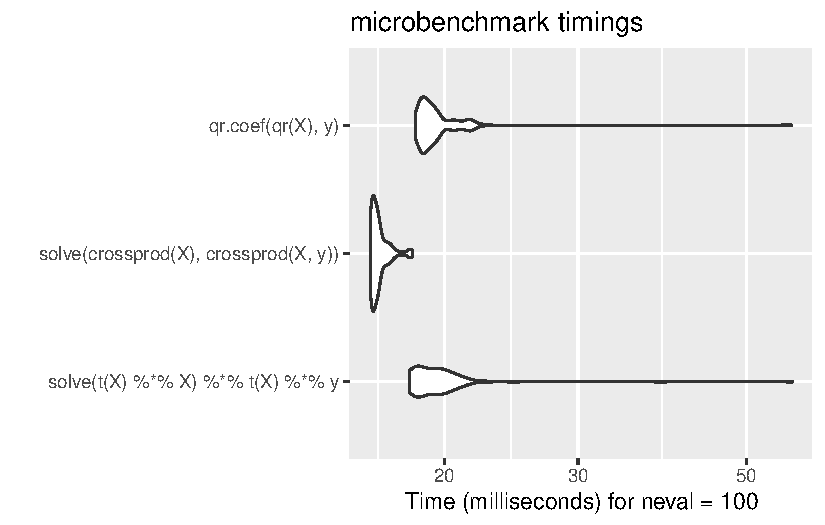
\includegraphics[keepaspectratio]{02-optimization_files/figure-pdf/unnamed-chunk-5-1.pdf}}

Compared with the approaches discussed above, this method performs
similarly to the naive approach but is much more stable and reliable.

In practice, we rarely call functions such as \texttt{qr()} or
\texttt{qr.coef()} directly, since higher-level functions like lm()
handle these computations automatically. However, in certain specialized
and performance-critical settings, it can be advantageous to use
alternative matrix decompositions to compute regression coefficients,
especially when the computation must be repeated many times in a loop
(i.e., \emph{Vectorization})

\subsection{Multivariate Normal
revisit}\label{multivariate-normal-revisit}

Computing the multivariate normal (MVN) density is a common task, for
example, when fitting spatial models or Gaussian process models. Because
maximum likelihood estimation(MLE) and likelihood ratio tests (LRT)
often require evaluating the likelihood many times, efficiency is
crucial.

After taking the log of the MVN density, we have

\[
\ell(\boldsymbol{x}\mid \boldsymbol{\mu},\Sigma) := \log \left\{ f(\boldsymbol{x}\mid \boldsymbol{\mu},\Sigma) \right\} 
= -\frac{d}{2}\log(2\pi) - \frac{1}{2}\log|\Sigma| - \frac{1}{2}(\boldsymbol{x}-\boldsymbol{\mu})^\top \Sigma^{-1}(\boldsymbol{x}-\boldsymbol{\mu}).
\] On the right hand side, the first term is a constant, the second term
is linear, and the last term is quadratic, which requires much more
computational power.

\subsubsection{A Naive Implementation}\label{a-naive-implementation}

We first center the data \(\boldsymbol{z}:=\boldsymbol{x}- \mu\). Then
we have \(\boldsymbol{z}^\top \Sigma^{-1} \boldsymbol{z}\). This
simiplified the question for a bit.

Here, much like the linear regression example above, the key bottleneck
is the inversion of the \(p\)-dimensional covariance matrix \(\Sigma\).
If we take \(\boldsymbol{z}\) to be a \(p\times 1\) column vector, then
a literal translation of the mathematics into R code might look
something like this,

\begin{Shaded}
\begin{Highlighting}[]
\FunctionTok{t}\NormalTok{(z) }\SpecialCharTok{\%*\%} \FunctionTok{solve}\NormalTok{(Sigma) }\SpecialCharTok{\%*\%}\NormalTok{ z}
\end{Highlighting}
\end{Shaded}

To illustrate, let's simulate some data and compute the quadratic form
the naive way:

\begin{Shaded}
\begin{Highlighting}[]
\FunctionTok{set.seed}\NormalTok{(}\DecValTok{2025{-}09{-}03}\NormalTok{)}

\CommentTok{\# Generate data}
\NormalTok{z }\OtherTok{\textless{}{-}} \FunctionTok{matrix}\NormalTok{(}\FunctionTok{rnorm}\NormalTok{(}\DecValTok{200} \SpecialCharTok{*} \DecValTok{100}\NormalTok{), }\DecValTok{200}\NormalTok{, }\DecValTok{100}\NormalTok{)}
\NormalTok{S }\OtherTok{\textless{}{-}} \FunctionTok{cov}\NormalTok{(z)}

\CommentTok{\# Naive quadratic form}
\NormalTok{quad.naive }\OtherTok{\textless{}{-}} \ControlFlowTok{function}\NormalTok{(z, S) \{}
\NormalTok{  Sinv }\OtherTok{\textless{}{-}} \FunctionTok{solve}\NormalTok{(S)}
  \FunctionTok{rowSums}\NormalTok{((z }\SpecialCharTok{\%*\%}\NormalTok{ Sinv) }\SpecialCharTok{*}\NormalTok{ z)}
\NormalTok{\}}

\FunctionTok{library}\NormalTok{(dplyr)}
\FunctionTok{quad.naive}\NormalTok{(z, S) }\SpecialCharTok{\%\textgreater{}\%} \FunctionTok{summary}\NormalTok{()}
\end{Highlighting}
\end{Shaded}

\begin{verbatim}
   Min. 1st Qu.  Median    Mean 3rd Qu.    Max. 
  70.67   93.61   99.94  100.54  107.31  126.73 
\end{verbatim}

\subsubsection{A Better Way: Cholesky
Decomposition}\label{a-better-way-cholesky-decomposition}

Because the covariance matrix \Sigma is symmetric and positive definite,
we can exploit its \textbf{Cholesky decomposition}. That is, we write
\(\Sigma = R^\top R\), where \(R\) is a upper triangular matrix. Then,
\[
\boldsymbol{z}^\top \Sigma^{-1} \boldsymbol{z}= \boldsymbol{z}^\top (R^\top R)^{-1} \boldsymbol{z}= \boldsymbol{z}^\top R^{-1}R^{-\top} \boldsymbol{z}= (R^{-\top}\boldsymbol{z})^\top (R^{-\top} \boldsymbol{z}) := \boldsymbol{v}^\top \boldsymbol{v}.
\] Note that \(\boldsymbol{v}\in \mathbb R^p\) is the solution to the
linear system \(R^\top \boldsymbol{v}= \boldsymbol{z}\). Because \(R\)
is upper triangular, we can solve this system efficiently using back
substitution. Also, we can solve this without doing the inversion.

Once we have \(\boldsymbol{v}\) we can compute its quadratic form
\$\boldsymbol{v}\^{}\top \boldsymbol{v} \$ by the \texttt{crossprod()}
function.

\begin{Shaded}
\begin{Highlighting}[]
\NormalTok{quad.chol }\OtherTok{\textless{}{-}} \ControlFlowTok{function}\NormalTok{(z, S) \{}
\NormalTok{  R }\OtherTok{\textless{}{-}} \FunctionTok{chol}\NormalTok{(S)}
\NormalTok{  v }\OtherTok{\textless{}{-}} \FunctionTok{backsolve}\NormalTok{(R, }\FunctionTok{t}\NormalTok{(z), }\AttributeTok{transpose =} \ConstantTok{TRUE}\NormalTok{)}
  \FunctionTok{colSums}\NormalTok{(v }\SpecialCharTok{*}\NormalTok{ v)}
\NormalTok{\}}

\FunctionTok{quad.chol}\NormalTok{(z, S) }\SpecialCharTok{\%\textgreater{}\%} \FunctionTok{summary}\NormalTok{()}
\end{Highlighting}
\end{Shaded}

\begin{verbatim}
   Min. 1st Qu.  Median    Mean 3rd Qu.    Max. 
  70.67   93.61   99.94  100.54  107.31  126.73 
\end{verbatim}

\subsubsection{By product}\label{by-product}

Another benefit of the Cholesky decomposition is that it gives us a
simple way to compute the log-determinant of \(\Sigma\). The
log-determinant of \(\Sigma\) is simply two times the sum of the log of
the diagonal elements of R. (Why?)

\subsubsection{Performance comparison}\label{performance-comparison}

\begin{Shaded}
\begin{Highlighting}[]
\FunctionTok{library}\NormalTok{(microbenchmark)}
\FunctionTok{library}\NormalTok{(ggplot2)}
\NormalTok{m2 }\OtherTok{\textless{}{-}} \FunctionTok{microbenchmark}\NormalTok{(}
  \AttributeTok{naive =} \FunctionTok{quad.naive}\NormalTok{(z, S),}
  \AttributeTok{chol  =} \FunctionTok{quad.chol}\NormalTok{(z, S)}
\NormalTok{)}
\FunctionTok{autoplot}\NormalTok{(m2)}
\end{Highlighting}
\end{Shaded}

\pandocbounded{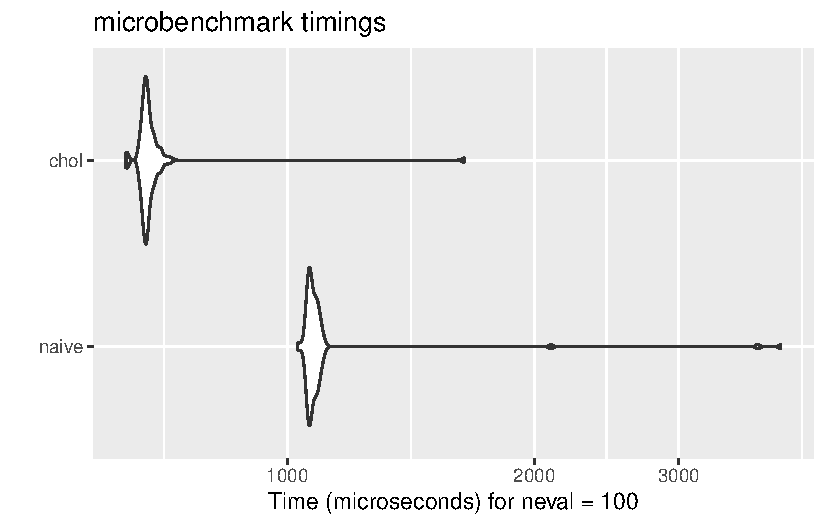
\includegraphics[keepaspectratio]{02-optimization_files/figure-pdf/unnamed-chunk-8-1.pdf}}

Q: Why one is faster than the other?

\subsubsection{Take home message 2}\label{take-home-message-2}

The naive algorithm simply inverts the covariance matrix. The
Cholesky-based approach, on the other hand, exploits the fact that
covariance matrices are symmetric and positive definite. This results in
an implementation that is both faster and numerically more
stable---exactly the kind of optimization that makes a difference in
real-world statistical computing.

Thus, a knowledge of statistics and numerical analysis can often lead to
better algorithms, often invaluable!

\begin{center}\rule{0.5\linewidth}{0.5pt}\end{center}

\section{We will touch the concept below in next
class}\label{we-will-touch-the-concept-below-in-next-class}

\section{Type of Optimization
Algorithms}\label{type-of-optimization-algorithms}

There are in general two types of the optimization algorithms: (1).
\textbf{deterministic} and (2). \textbf{metaheuristic}. Deterministic
and metaheuristic algorithms represent two distinct paradigms in
optimization. Deterministic methods, such as gradient descent, produce
the same solution for a given input and follow a predictable path toward
an optimum. In contrast, metaheuristic approaches---like genetic
algorithms---incorporate randomness and do not guarantee the best
possible solution. However, they are often more effective at avoiding
local optima and exploring complex search spaces.

\section{Heuristic Algorithms}\label{heuristic-algorithms}

Many of the heuristic algorithms are inspired by the nature, such as the
genetic algorithm (GA) and particle swarm optimization (PSO). These
algorithms are often used for complex optimization problems where
traditional methods may struggle to find a solution. Some of the popular
heuristic algorithms include:

\begin{itemize}
\tightlist
\item
  Genetic Algorithm (GA)
\item
  Particle Swarm Optimization (PSO)
\item
  Simulated Annealing (SA)
\item
  Ant Colony Optimization (ACO)
\end{itemize}

\section{Deterministic Algorithms}\label{deterministic-algorithms}

Numerical approximation, what you learned in the mathematical
optimization course. Some of the algorithms include:

\begin{itemize}
\tightlist
\item
  Gradient Descent
\item
  Newton's Method
\item
  Conjugate Gradient Method
\item
  Quasi-Newton Methods (e.g., BFGS)
\item
  Interior Point Methods
\end{itemize}

They often reply on the KKT conditions.

\subsection{In R}\label{in-r}

\texttt{optim()} function, \texttt{nlm()} function or \texttt{mle()}
function.

\subsection{EM Algorithm}\label{em-algorithm}

The EM (Expectation--Maximization) algorithm is an optimization method
that is often applied to find maximum likelihood estimates when data is
incomplete or has missing values. It iteratively refines estimates of
parameters by alternating between (1) expectation step (E-step) and (2)
maximization step (M-step).

\begin{tcolorbox}[enhanced jigsaw, arc=.35mm, toprule=.15mm, opacitybacktitle=0.6, bottomtitle=1mm, colbacktitle=quarto-callout-note-color!10!white, colback=white, bottomrule=.15mm, breakable, colframe=quarto-callout-note-color-frame, left=2mm, opacityback=0, toptitle=1mm, titlerule=0mm, leftrule=.75mm, coltitle=black, rightrule=.15mm, title=\textcolor{quarto-callout-note-color}{\faInfo}\hspace{0.5em}{Tip with Title}]

For example, consider the function \(f(x) = x^2\).

\end{tcolorbox}

Example

\[
f(x) = x^2
\]

Example Theorem

\begin{center}\rule{0.5\linewidth}{0.5pt}\end{center}

Examples are borrowed from the following sources:

\begin{itemize}
\tightlist
\item
  Peng, R.D. \href{https://bookdown.org/rdpeng/advstatcomp/}{Advanced
  Statistical Computing}.
\end{itemize}

\bookmarksetup{startatroot}

\chapter{Resampling, Jackknife and
Bootstrap}\label{resampling-jackknife-and-bootstrap}

\newcommand{\bx}{\mathbf{x}}

\section{Introduction}\label{introduction}

This chapter covers resampling methods including the jackknife and
bootstrap techniques.

\section{Jackknife}\label{jackknife}

The jackknife is a resampling technique used to estimate the bias and
variance of a statistic.

Jackknife is like a \textbf{leave-one-out cross-validation}. Let
\(\mathbf{x}= (x_1,\dots,x_n)\) be an observed random sample, and denote
the \(i\)th jackknife sample by
\(\mathbf{x}_{-i} = (x_1,\dots,x_{i-1},x_{i+1},\dots,x_n)\), that is, a
subset of \(\mathbf{x}\).

For the parameter of interest \(\theta\), if the statistics is
\(T(\mathbf{x})=:\hat{\theta}\) is computed on the full

\subsection{When does jackknife not
work?}\label{when-does-jackknife-not-work}

Jackknife does not work when the function \(T(\cdot)\) is \textbf{not a
smooth} functional!

\section{Bootstrap}\label{bootstrap}

The bootstrap is a resampling method that allows estimation of the
sampling distribution of almost any statistic using random sampling
methods.

\section{Applications}\label{applications}

These methods are widely used in statistical inference and have
applications in various fields.

\begin{center}\rule{0.5\linewidth}{0.5pt}\end{center}

\bookmarksetup{startatroot}

\chapter{Additional Topics}\label{additional-topics}

This chapter covers additional topics that will only be going over if
time permits.

\section{High-dimensional data}\label{high-dimensional-data}

\section{Dimensional Reduction
Methods}\label{dimensional-reduction-methods}

\subsection{Principal Component
Analysis}\label{principal-component-analysis}

\bookmarksetup{startatroot}

\chapter*{References}\label{references}
\addcontentsline{toc}{chapter}{References}

\markboth{References}{References}

\phantomsection\label{refs}

\part{Appendix}

\chapter{Appendix: Introduction to R?}\label{appendix-introduction-to-r}

\section{R}\label{r}

For conducting analyses with data sets of hundreds to thousands of
observations, calculating by hand is not feasible and you will need a
statistical software. \textbf{R} is one of those. \textbf{R} can also be
thought of as a high-level programming language. In fact, \textbf{R} is
\href{https://statisticstimes.com/tech/top-computer-languages.php}{one
of the top languages} to be used by data analysts and data scientists.
There are a lot of analysis packages in \textbf{R} that are currently
developed and maintained by researchers around the world to deal with
different data problems. Most importantly, \textbf{R} is free! In this
section, we will learn how to use \textbf{R} to conduct basic
statistical analyses.

\section{IDE}\label{ide}

\subsection{Rstudio}\label{rstudio}

RStudio is an integrated development environment (IDE) designed
specifically for working with the \textbf{R} programming language. It
provides a user-friendly interface that includes a source editor,
console, environment pane, and tools for plotting, debugging, version
control, and package management. RStudio supports both \textbf{R} and
Python and is widely used for data analysis, statistical modeling, and
reproducible research. It also integrates seamlessly with tools like
\textbf{R} Markdown, Shiny, and Quarto, making it popular among data
scientists, statisticians, and educators.

\subsection{Visual Studio Code (VS
Code)}\label{visual-studio-code-vs-code}

VS Code is a versatile code editor that supports multiple programming
languages, including \textbf{R}. With the \textbf{R} extension for VS
Code, users can write and execute \textbf{R} code, access \textbf{R}'s
console, and utilize features like syntax highlighting, code completion,
and debugging. While not as specialized as RStudio for \textbf{R}
development, VS Code offers a lightweight alternative with extensive
customization options and support for various programming tasks.

\subsection{Positron}\label{positron}

Positron IDE is the next-generation integrated development environment
developed by Posit, the company behind RStudio. Designed to be a modern,
extensible, and language-agnostic IDE, Positron builds on the strengths
of RStudio while supporting a broader range of languages and workflows,
including \textbf{R}, Python, and Quarto.

\section{RStudio Layout}\label{rstudio-layout}

RStudio consists of several panes: - \textbf{Source}: Where you write
scripts and markdown documents. - \textbf{Console}: Where you type and
execute \textbf{R} commands. - \textbf{Environment/History}: Shows your
variables and command history. -
\textbf{Files/Plots/Packages/Help/Viewer}: For file management, viewing
plots, managing packages, accessing help, and viewing web content.

\section{R Scripts}\label{r-scripts}

\textbf{R} scripts are plain text files containing \textbf{R} code. You
can create a new script in RStudio by clicking
\texttt{File\ \textgreater{}\ New\ File\ \textgreater{}\ R\ Script}.

\section{R Help}\label{r-help}

Use \texttt{?function\_name} or \texttt{help(function\_name)} to access
help for any \textbf{R} function. For example:

\begin{Shaded}
\begin{Highlighting}[]
\NormalTok{?mean}
\FunctionTok{help}\NormalTok{(mean)}
\end{Highlighting}
\end{Shaded}

\section{R Packages}\label{r-packages}

Packages extend \textbf{R}'s functionality. There are thousands of
packages available in \textbf{R} ecosystem. You may install them from
different sources.

\subsection{With Comprehensive R Archive Network
(CRAN)}\label{with-comprehensive-r-archive-network-cran}

CRAN is the primary repository for \textbf{R} packages. It contains
thousands of packages that can be easily installed and updated.

Install a package with:

\begin{Shaded}
\begin{Highlighting}[]
\FunctionTok{install.packages}\NormalTok{(}\StringTok{"package\_name"}\NormalTok{)}
\end{Highlighting}
\end{Shaded}

\subsection{With Bioconductor}\label{with-bioconductor}

Bioconductor is a repository for bioinformatics packages in \textbf{R}.
It provides tools for the analysis and comprehension of high-throughput
genomic data.

Install Bioconductor packages using the \texttt{BiocManager} package:

\begin{Shaded}
\begin{Highlighting}[]
\NormalTok{BiocManager}\SpecialCharTok{::}\FunctionTok{install}\NormalTok{(}\StringTok{"package\_name"}\NormalTok{)}
\end{Highlighting}
\end{Shaded}

\subsection{From GitHub}\label{from-github}

Many of the authors of \textbf{R} packages host their work on GitHub.
You can install these packages using the \texttt{devtools} package:

\begin{Shaded}
\begin{Highlighting}[]
\NormalTok{devtools}\SpecialCharTok{::}\FunctionTok{install\_github}\NormalTok{(}\StringTok{"username/package\_name"}\NormalTok{)}
\end{Highlighting}
\end{Shaded}

\subsection{Load a package}\label{load-a-package}

Once a package is installed, you need to load it into your \textbf{R}
session to use its functions:

\begin{Shaded}
\begin{Highlighting}[]
\FunctionTok{library}\NormalTok{(package\_name)}
\end{Highlighting}
\end{Shaded}

Alternatively, you may use a function in the package with
\texttt{package\_name::function\_name()} without loading the entire
package.

\section{R Markdown}\label{r-markdown}

\textbf{R} Markdown allows you to combine text, code, and output in a
single document. Create a new \textbf{R} Markdown file in RStudio via
\texttt{File\ \textgreater{}\ New\ File\ \textgreater{}\ R\ Markdown...}.

Recently, the posit team has developed a new version of the \textbf{R}
Markdown called quarto document, with the file extension \texttt{.qmd}.
It is still under rapid development.

\section{Vectors}\label{vectors}

Vectors are the most basic data structure in \textbf{R}.

\begin{Shaded}
\begin{Highlighting}[]
\NormalTok{x }\OtherTok{\textless{}{-}} \FunctionTok{c}\NormalTok{(}\DecValTok{1}\NormalTok{, }\DecValTok{2}\NormalTok{, }\DecValTok{3}\NormalTok{, }\DecValTok{4}\NormalTok{, }\DecValTok{5}\NormalTok{)}
\NormalTok{x}
\end{Highlighting}
\end{Shaded}

\begin{verbatim}
[1] 1 2 3 4 5
\end{verbatim}

You can perform operations on vectors:

\begin{Shaded}
\begin{Highlighting}[]
\NormalTok{x }\SpecialCharTok{*} \DecValTok{2}
\end{Highlighting}
\end{Shaded}

\begin{verbatim}
[1]  2  4  6  8 10
\end{verbatim}

\section{Data Sets}\label{data-sets}

Data frames are used for storing data tables. Create a data frame:

\begin{Shaded}
\begin{Highlighting}[]
\NormalTok{df }\OtherTok{\textless{}{-}} \FunctionTok{data.frame}\NormalTok{(}\AttributeTok{Name =} \FunctionTok{c}\NormalTok{(}\StringTok{"Alice"}\NormalTok{, }\StringTok{"Bob"}\NormalTok{), }\AttributeTok{Score =} \FunctionTok{c}\NormalTok{(}\DecValTok{90}\NormalTok{, }\DecValTok{85}\NormalTok{))}
\NormalTok{df}
\end{Highlighting}
\end{Shaded}

\begin{verbatim}
   Name Score
1 Alice    90
2   Bob    85
\end{verbatim}

You can import data from files using \texttt{read.csv()} or
\texttt{read.table()}.

\begin{center}\rule{0.5\linewidth}{0.5pt}\end{center}

This appendix is adapted from
\href{https://tqtbui.github.io/introbook/app-rintro.html}{Why R?}.




\end{document}
